% !TeX root = t3_3000.tex

\documentclass[a4paper,10pt]{article}

% Sprache / Kodierung
\usepackage[ngerman]{babel}
\usepackage[T1]{fontenc}
\usepackage{csquotes}

% Schrift
\usepackage{newtxtext,newtxmath} % Times-ähnlich

% Seitenlayout
\usepackage[a4paper,margin=2.2cm]{geometry}
\setlength{\parindent}{0pt}
\setlength{\parskip}{0pt}

% Mehrspaltig ohne Kontrolle
\usepackage{multicol}
\usepackage{stfloats}

% Sonstiges
\usepackage{graphicx}
\usepackage{enumitem}
\usepackage[hidelinks]{hyperref}
\usepackage{svg}
\usepackage{pdfpages}

\usepackage{caption}
\usepackage[x11names]{xcolor}

\captionsetup{font={small, color=SlateGray4}}

\usepackage[backend=biber, style=authoryear]{biblatex}
\addbibresource{quellen.bib}

% use [] for parencites
\makeatletter
\DeclareFieldFormat{citebackslash}{[\mkbibnamelast{#1}]}
\renewcommand*{\nameyeardelim}{\addcomma\space} % Adds comma like [Jones, 2024]
\DeclareFieldFormat{biblabeldate}{#1}
\DeclareCiteCommand{\parencite}[\mkbibbrackets]
  {\usebibmacro{prenote}}
  {\usebibmacro{citeindex}%
   \usebibmacro{cite}}
  {\multicitedelim}
  {\usebibmacro{postnote}}
\makeatother

% Überschriften enger und zentriert
\usepackage{titlesec}
\titleformat{\section}
{\normalfont\large\bfseries\centering}
{}
{0pt}
{}
\titleformat{\subsection}
{\normalfont\normalsize\bfseries}
{}
{0pt}
{}
\titlespacing*{\section}{0pt}{1.2em}{0.6em}
\titlespacing*{\subsection}{0pt}{0.8em}{0.3em}

% Literaturüberschrift ohne Nummer
\renewcommand{\refname}{Literatur}

\begin{document}

	% header
	% !TeX root = t3_3000.tex

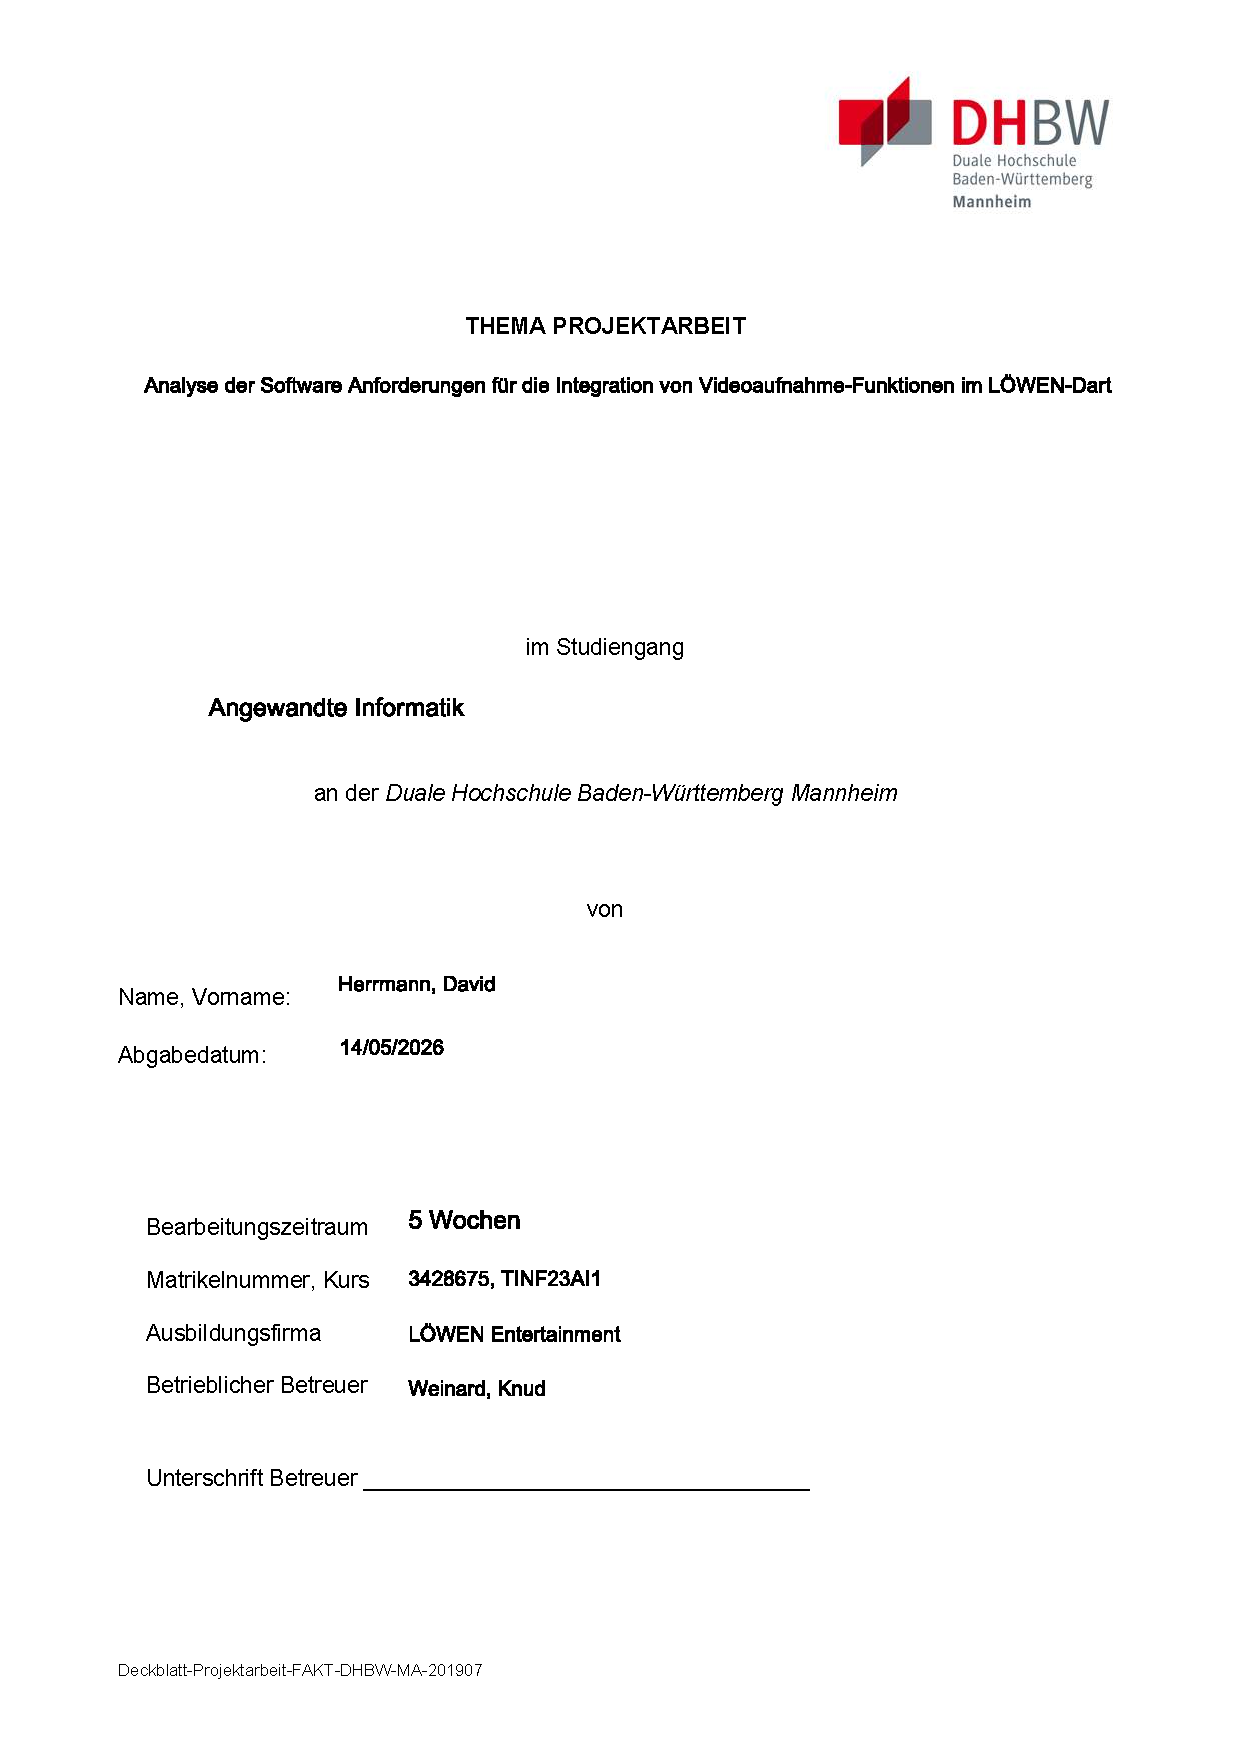
\includepdf[pages=1]{Head/DeckblattPrinted.pdf}

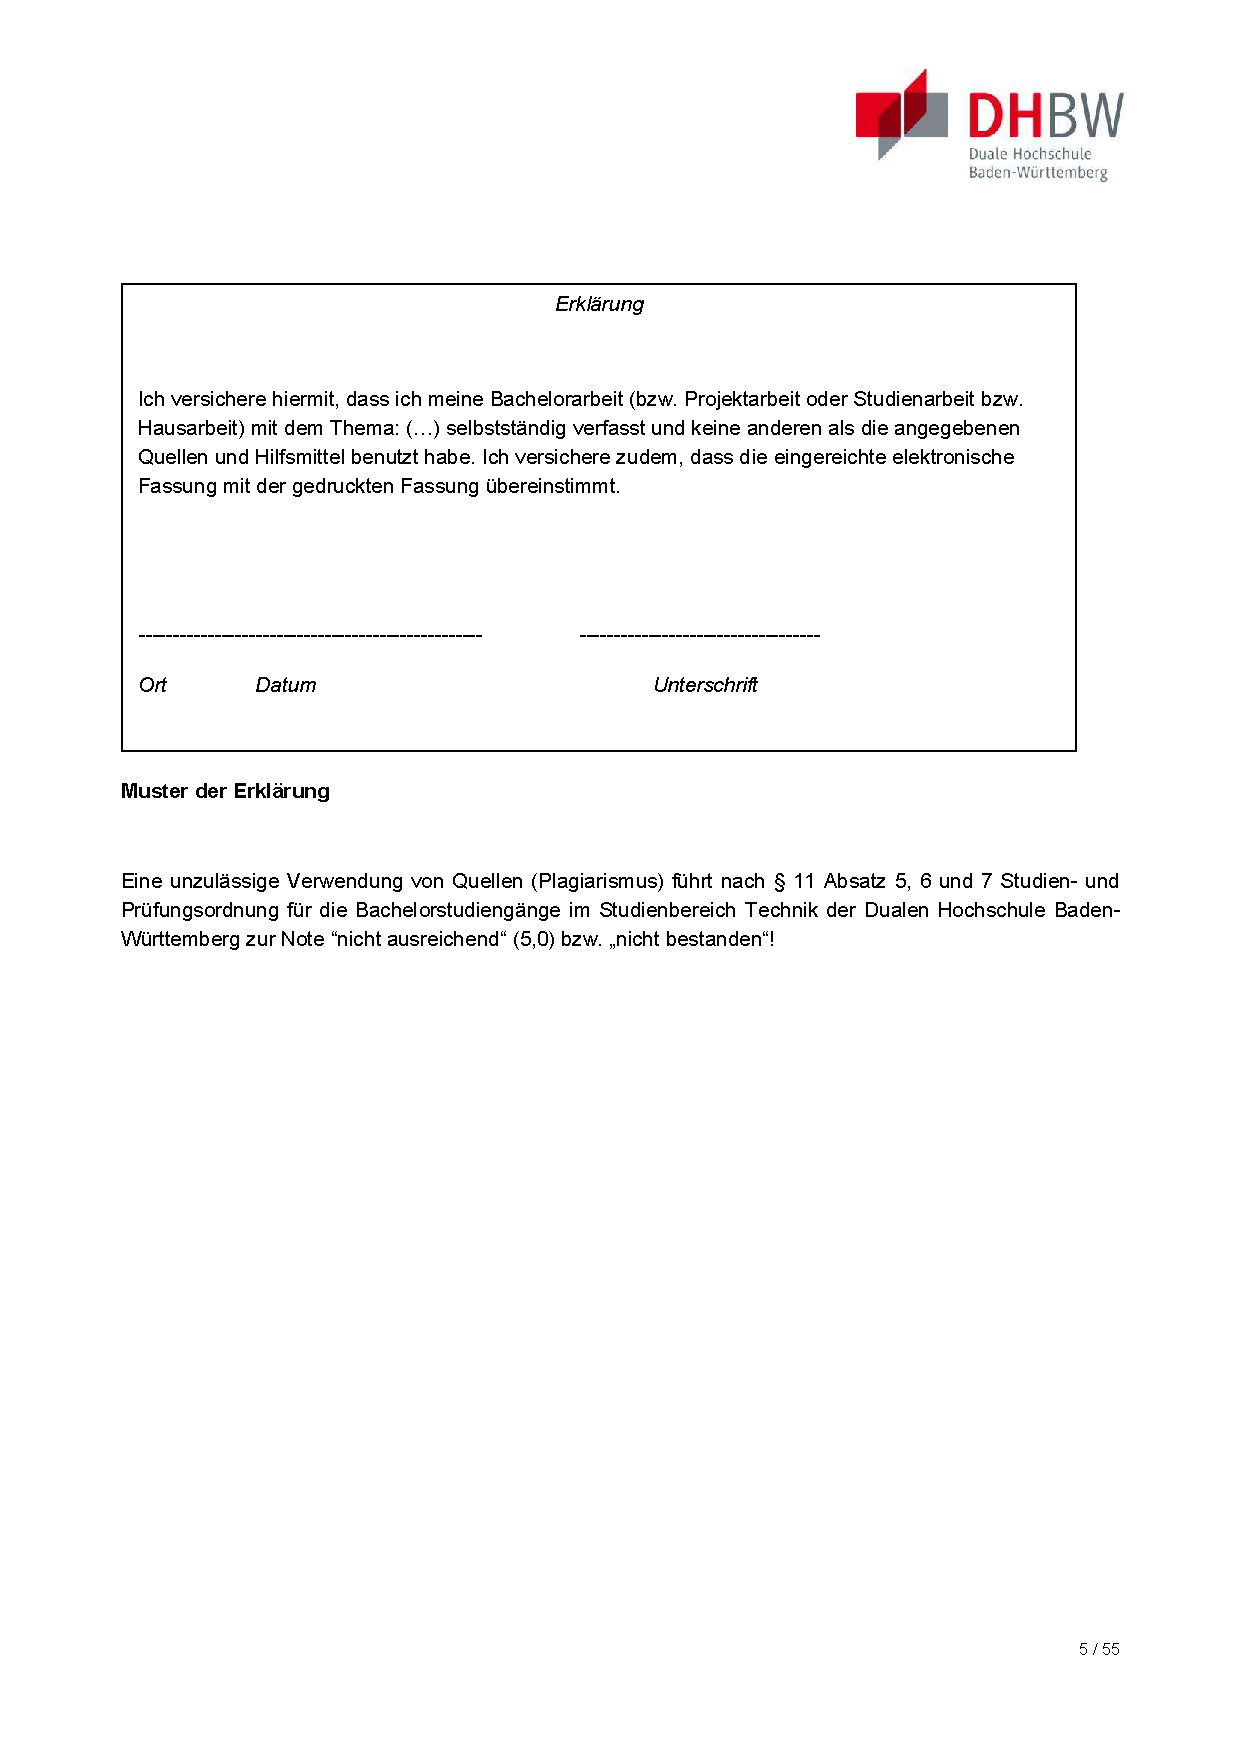
\includepdf[pages=1]{Head/Selbstständigkeitserklärung.pdf}
	
	\setcounter{page}{1}

	% Zentrierter Titelblock
	\begin{center}
		{\LARGE\bfseries Analyse der Software Anforderungen für die Integration von Videoaufnahme-Funktionen im LÖWEN-Dart\par}
		\vspace{0.8cm}
		
		{\large\bfseries David Herrmann\par}
		\vspace{0.2cm}
		
		3428675, LÖWEN ENTERTAINMENT\par
		s231259@student.dhbw-mannheim.de
	\end{center}
	
	\vspace{0.8cm}
	
	% Zweispaltiger Hauptteil
	\begin{multicols*}{2}
	
		%Zusammenfassung
		% !TeX root = t3_3000.tex

{
\titleformat{\subsection}[block]{\normalfont\normalsize\bfseries\filcenter}{}{0pt}{}
	\subsection*{Abstract}

	\begin{quote}
	{\fontsize{9}{11}\selectfont
		Diese Arbeit befasst sich mit den softwareseitigen Anforderungen für die Integration einer Videofunktion in das HB10 E-Dart Gerät, um die sportliche Integrität bei online Wettbewerben sicherzustellen. 
		Der Fokus liegt auf der Untersuchung ressourceneffizienter Methoden für den Kamerazugriff unter Linux mittels der Video for Linux API sowie der performanten Videokomprimierung durch 
		hardwarebeschleunigte Codecs zur Entlastung von Prozessor und Arbeitsspeicher. Des Weiteren werden Algorithmen zur automatisierten Erkennung von Manipulationsversuchen betrachtet. 
		Abschließend erfolgt eine Analyse von Übertragungsverfahren für die Übertragung von Videos an einen Server zur Speicherung, 
		mit Fokus auf die Minimierung der benötigten Bandbreite und CPU-Auslastung des Servers.
	}
	\end{quote}
	

	\vspace{1.2em}
}

		%Einleitung
		% !TeX root = t3_3000.tex

\section{Einleitung}

Das E-Dart Gerät \textit{LÖWEN DART HB10} stellt ein System dar, das bereits umfangreiche Funktionen für den Spielbetrieb bietet \parencite{lwenentertainment_2026_lwen}. Hierzu zählen neben dem Bereitstellung verschiedener Dart-Spiele die Erfassung von Spielerstatistiken 
die Bereitstellung von Daten über eine mobile Applikation sowie ein Verwaltungsportal für Aufsteller. Ein zentraler Aspekt des aktuellen Betriebs sind die \textit{3K}-Turniere, bei denen alle Teilnehmer zeitgleich an demselben Gerät agieren 
und die Spielergebnisse direkt nach Abschluss der Partie übertragen werden.\newline

In Zukunft soll dieses System um asynchrone Turnierformate und Ranglisten ergänzt werden, bei denen die Möglichkeit besteht, Preisgelder zu gewinnen. Im Gegensatz zu den bestehenden Formaten ist hierbei keine gleichzeitige Anwesenheit der Spieler erforderlich. 
Da die Wettbewerbe ortsungebunden durchgeführt werden können, ist eine visuelle Überprüfung der sportlichen Integrität erforderlich. Um Manipulationen am Spielausgang zu verhindern, wird eine Funktion zur Videoaufnahme der Spieler sowie der Dartscheibe benötigt. 
Da diese Kamerasysteme bisher nicht installiert sind, müssen geeignete Wege zur Integration gefunden werden, um die Aufnahmen zur Validierung an einen zentralen Server zu senden.\newline

Ziel dieser Arbeit ist die Untersuchung effizienter Methoden zur Implementierung dieser Videofunktionalität auf dem HB10. 
Der Fokus liegt hierbei auf einem ressourcenschonenden Zugriff auf die Aufnahmen der Kameras sowie einer performanten Kompression zur Entlastung von Prozessor und 
Arbeitsspeicher während der Verarbeitung. Des Weiteren wird untersucht, inwieweit simple Algorithmen zur automatisierten Erkennung von Manipulationsversuchen, wie die Entfernung des Spielers zur Scheibe,
in das System integriert werden können. Ein zentraler Aspekt der Untersuchung betrifft die Optimierung der Videoübertragung an einen Server. 
Hierbei werden Verfahren evaluiert, die sowohl die benötigte Bandbreite als auch die CPU-Auslastung des Servers minimieren, um einen ökonomischen und stabilen Betrieb sicher zu stellen.

\vspace{1em}


		
		%Kapitel 1: Video einlesen, und Kompression
		% !TeX root = t3_3000.tex

\begin{figure*}[!b]
    \centering
    \includesvg[width=\textwidth]{Images/Ringbuffer.svg}
    \caption{Das Diagramm zeigt, wie die Videodaten von der Videoquelle (Kamera) zum Endpunkt (Server) verlaufen könnten: Es werden die Videodaten der Kamera in dem rohen Format YUYV an den HB10 weitergegeben, 
             welcher immer etwa 3 Sekunden dieser Daten in einem Ringbuffer speichert. Bei einem Treffer mit dem Dart (Trigger) werden die Daten zunächst verarbeitet und anschließend komprimiert.
             Schließlich sendet der HB10 die komprimierten Videos an den Server. YUYV wurde als initiales Videoformat gewählt, da somit auf die Dekodierung der Videodaten innerhalb des HB10 verzichtet werden kann.}
    \label{fig:ringbuffer}
\end{figure*}

\section{Video- Aufnahme und Komprimierung} \label{sec:1}

Die Realisierung einer stabilen Videoaufnahme für den HB10 erfordert eine performante Interaktion zwischen Hardware und Software. Da die hohen Datenraten unkomprimierter Videostreams eine stabile und starke Internetverbindung voraussetzen, 
was nicht bei jedem Aufsteller eines HB10 der Fall ist, wird eine Komprimierung der Daten benötigt.\newline

Zur Minimierung der Prozessorlast und des Arbeitsspeicherverbrauchs bieten sich innerhalb der Linux-Umgebung hardwaregestützte Kodierungsverfahren an. Diese verlagern die rechenintensiven Kompressionsalgorithmen vom Hauptprozessor auf 
dedizierte Hardwareeinheiten \parencite{_2026_ffmpeg}. Dies ist insbesondere im Kontext der im HB10 eingebauten APU relevant, 
da diese über spezielle Funktionen zur beschleunigten Videoverarbeitung verfügt \parencite{_r1000, gpuopenlibrariessdks_2025_amf_video_encode_api}. Des Weiteren, ist es auch nicht nötig, den gesamten Spielablauf aufzunehmen. 
Es ist ausreichend, Videoausschnitte der einzelnen Würfe zu speichern. Im Folgenden werden die technischen Grundlagen des Kamerazugriffs sowie die Auswahl geeigneter Kompressionsverfahren unter Berücksichtigung der Hardwarebeschleunigung erläutert.

\subsection{Video-Komprimierungsalgorithmen} \label{sec:compression}

In der Videoverarbeitung wird grundlegend zwischen Intra-Frame- und Inter-Frame-Komprimierung unterschieden. Bei der Intra-Frame-Komprimierung wird jedes Bild einzeln bearbeitet. Hierbei lassen sich Daten einsparen, 
indem Informationen innerhalb eines Bildes zusammengefasst oder Details entfernt werden, die das menschliche Auge kaum wahrnehmen kann. Ein Beispiel hierfür ist der \textit{MJPEG}-Standard, 
der das \textit{YCbCr}-Farbmodell verwendet. Dabei wird die Helligkeit detailliert gespeichert, während die Farbinformationen reduziert werden \parencite{pearson_an}. \newline

Zusätzlich kann die Inter-Frame-Komprimierung genutzt werden, um die zeitlichen Ähnlichkeiten zwischen aufeinanderfolgenden Bildern zu verwenden. Anstatt jedes Bild vollständig zu speichern,
werden oft nur die Unterschiede zum vorherigen Bild aufgezeichnet \parencite{putra_2023_interframe}. Der Standard \textit{H.264} setzt dieses Prinzip durch \textit{I-Frames} und \textit{P-Frames} um. 
Während ein I-Frame das gesamte Bild enthält, speichern die folgenden P-Frames lediglich die Veränderungen zum vorangegangenen Bild \parencite{kalva_the}. Dieses
Vorgehen reduziert die Datenmenge sowie die benötigte Bandbreite erheblich.

\subsection{Hardwaregestützte Komprimierung} \label{sec:hwComp}

Das HB10 besitzt einen AMD Ryzen Embedded R1000 Prozessor als APU und ist ein Linux-basiertes System. Die vorgesehene Kamera (Modell: ELP-USB3MP01H-L29) unterstützt die Video Formate MJPEG \textit{YUYV} und H.264 in verschiedenen Auflösungen und Wiederholraten,
in Abhängigkeit der Formate.\newline

Da die Videofunktion im Hintergrund des eigentlichen Spiels ablaufen soll, darf die Komprimierung nur einen kleinen Teil der CPU-Leistung beanspruchen. Dazu kann man den Grafikprozessors verwenden, da dieser deutlich effizienter bei der Durchführung von Video-Komprimierung ist. 
Der Grafikprozessor des HB10 unterstützt die \textit{Video Core Next} (VCN) Engine von AMD  \parencite{_2025_amd,_r1000}.\newline

Die in der APU integrierte VCN-Einheit stellt dedizierte Hardware-Encoder für Formate wie H.264 bereit, wodurch die Rechenlast von den CPU-Kernen auf spezialisierte Hardwarekomponenten verlagert 
wird \parencite{_r1000, _2025_amd}. Für die Umsetzung unter Linux kann die \textit{Video Acceleration API} (VA-API) als Schnittstelle genutzt werden \parencite{_2026_ffmpeg}. Diese erlaubt es, 
die Hardwarebeschleunigung der APU direkt anzusprechen, um Videoströme mit minimalem Ressourcenverbrauch zu kodieren.

\subsection{Kamera als Videoquelle} \label{sec:camera}

Bisher gab es keine Notwendigkeit für eine Kamera am HB10, deshalb besteht noch keine Schnittstelle für den Zugriff auf diese.
Der Zugriff erfolgt unter Linux standardmäßig über die \textit{Video for Linux} (V4L) Schnittstelle des Kernels \parencite{_2020_part}. Diese API ermöglicht eine direkte Kommunikation mit dem Videogerät, 
erfordert jedoch eine komplexe Handhabung der Puffer und Formate. Um die Implementierung effizienter zu gestalten, könnte man auf das Framework \textit{FFmpeg} zurückgegriffen \parencite{_2018_ffmpeg}. FFmpeg dient als Abstraktionsebene für V4L und 
vereinfacht den Prozess der Videoaufnahme erheblich \parencite{_documentation}. Des Weiteren kann FFmpeg auch für den Zugriff auf die Codecs des Grafikprozessors verwendet werden.\newline

Da das verwendete Kamera Modell komprimierte Video-Formate unterstützt, besteht die Möglichkeit, diese zu verwenden. In unserem Fall möchten wir die Videos aber weiterverarbeiten, 
deshalb empfiehlt sich die Verwendung unkomprimierter Formate, um den Rechenaufwand für eine Dekomprimierung zu vermeiden. Des Weiteren ist es vorgesehen, die Videos auf dem HB10 in einem Ringbuffer zu Speichern (siehe Abbildung \ref{fig:ringbuffer}). Unter der Verwendung komprimierter Video-Formate ist es aber schwierig die Ringbuffer Größe zu definieren,
da jeder einzelne Frame unterschiedlich groß ist, und bei Formaten die Intra-frame-Kompression verwenden, nicht garantiert werden kann, dass zu jeden Zeitpunkt ein vollständiger I-Frame im Buffer enthalten ist.

Das Kamera-Modell, dass eingebaut werden soll unterstützt als unkomprimiertes Format das YUYV-Pixelformat, dieses kann also für die Verarbeitung innerhalb des HB10 verwendet werden, für die Übertragung an den Server sollte ein komprimiertes Format gewählt werden.

\subsection{Analyse der Kompressionsverfahren MJPEG, H.264 und H.265}

Die Auswahl eines geeigneten Kompressionsverfahrens für dieÜbertragung an den Server, ist entscheidend für die Balance zwischen der Auslastung lokaler Ressourcen und der benötigten Netzwerkbandbreite. Da wir ein unkomprimiertes Videoformat für die Verarbeitung auf dem HB10 verwenden, 
spielen die restlichen Formate der Kamera keine Rolle, sondern entscheidend ist, welche Formate von dem Grafikprozessor kodiert werden können. Der Grafikprozessor des HB10 unterstützt die Komprimierung in die Formate H.264 und H.265.\newline

H.264 und H.265 nutzen die Inter-Frame-Kompression, um Redundanzen über die Zeit hinweg zu reduzieren \parencite{putra_2023_interframe}. H.264 bietet eine weitreichende Kompatibilität und eine 
effiziente Reduktion der Dateigröße\parencite{kalva_the}. Da die Hardware des Typs AMD Ryzen Embedded R1000 dieses Format unterstützt, könnte die Kompression 
mittels VA-APIdirekt auf die GPU ausgelagert werden \parencite{_2026_ffmpeg, gpuopenlibrariessdks_2025_amf_video_encode_api}. Dies schont die CPU-Ressourcen und den Arbeitsspeicher während des Betriebs \parencite{_2025_amd}.\newline

H.265 erreicht bei gleicher visueller Qualität eine noch stärkere Kompression als H.264, was die benötigte Bandbreite für die Übertragung an einen Server weiter minimiert \parencite{putra_2023_interframe}. Allerdings ist 
die algorithmische Komplexität von H.265 deutlich höher. Dieses Format ist sinnvoll, wenn die Einsparung von Speicherplatz und Rechenleistung auf dem Server und die Reduktion der Übertragungskosten Vorrang vor der minimalen Latenz auf dem lokalen Gerät haben.\newline

Für die Übertragung an den Server bietet sich H.265 an, da es die benötigte Bandbreite im Vergleich zu den anderen Formaten am besten reduziert.

\vspace{1em}
		
		%Kapitel 2: Spieler Erkennung
		% !TeX root = t3_3000.tex
        
\section{Effiziente Objekterkennung zur Analyse am Dart-Gerät}

Um eine automatisierte Prüfung des Wurfabstands sowie eine Unterscheidung zwischen geworfenen und gesteckten Pfeilen umzusetzen, ist eine ressourcenschonende Objekterkennung notwendig. 
Durch die Lokalisierung des Spielers im Kamerabild kann mathematisch geprüft werden, ob die Distanz zum Dart-Gerät in etwa den Regeln entspricht. Um den Anforderungen an eine geringe CPU- und Arbeitsspeicherauslastung auf der Zielhardware gerecht zu werden, 
müssen die untersuchten Verfahren eine niedrige algorithmische Komplexität aufweisen \parencite{_14, _2025_amd}.\newline

Techniken wie \enquote{Support Vector Machines} (SVM) in zusammenarbeit mit \enquote{Histogram of Oriented Gradients} (HOG) sind dabei vorteilhaft, da sie die CPU weniger belasten als tiefe neuronale Netze \parencite{_14}. Dies stellt sicher, dass die Hardware, 
genügend Kapazitäten für den zeitgleichen Spielbetrieb und die Videoverarbeitung behält \parencite{_2025_amd}.
		

		%Kapitel 3: Video Übertragung
		% !TeX root = t3_3000.tex

\section{Übertragung an einen Server}

Die Übermittlung der erfassten Videodaten an eine Serverinstanz stellt eine zentrale Herausforderung für die Effizienz des Gesamtsystems dar. Ein primäres Forschungsziel ist die Minimierung der Bandbreitennutzung bei der Übertragung. Davon entkoppelt 
ist die Anforderung, die Rechenlast auf dem Server so gering wie möglich zu halten, was durch eine clientseitige Vorverarbeitung und Kompression erreicht werden kann. \newline

Da die spezifische Serverart derzeit noch nicht definiert ist, kommen verschiedene Übertragungsmodelle in Betracht. Für eine dateibasierte Speicherung in einem \enquote{Object Storage} \parencite{susnjara_2025_object} bieten sich Verfahren wie 
\enquote{multipart/form-data} \parencite{muhibullah_2024_understanding} oder das \enquote{Secure Copy Protocol} \parencite{_2020_scp} an. Alternativ könnten Streaming-Protokolle wie \enquote{SRT} \parencite{haivision_2025_srtdocsreadmemd} oder 
\enquote{RTMP} \parencite{_2023_was} für eine kontinuierliche Datenübermittlung untersucht werden.

		%Fazit
		% !TeX root = t3_3000.tex

\section{Schlussbetrachtung}

Die vorliegende Untersuchung zeigt theoretische Möglichkeiten auf, eine ressourceneffiziente Videoverarbeitungskette unter Linux zu realisieren. Ein direkter Zugriff auf USB-Kameras ist mittels \textit{ffmpeg} möglich. Um CPU und RAM zu entlasten, bietet sich die hardwarebeschleunigte Enkodierung mittels \textit{VA-API} an, welche speziell auf Hardware wie der 
AMD Ryzen R1000 Serie effizient operiert.\newline

Für die Detektion von Spielern stellen Histogram of Oriented Gradients in Verbindung mit Support Vector Machines einen bewährten, rechenarmen Ansatz dar. 
Die anschließende Übertragung an einen Server kann mittels Übertragung über REST-Schnittstellen an einen Object-Storage Server realisiert werden.

\vspace{1em}
		
		%Literatur usw.
				% !TeX root = t3_3000.tex
		
		\vspace{1.2em}
		
		\section*{Literatur}

        \printbibliography


		
	\end{multicols*}
	
\end{document}